\documentclass{beamer}
\usetheme{default}
\usepackage{thumbpdf}
\usepackage{wasysym}
\usepackage{ucs}
\usepackage[utf8]{inputenc}
\usepackage{pgf,pgfarrows,pgfnodes,pgfautomata,pgfheaps,pgfshade}
\usepackage{verbatim}
\usepackage{listings}
\usepackage{color}

\definecolor{dkgreen}{rgb}{0,0.6,0}
\definecolor{gray}{rgb}{0.5,0.5,0.5}
\definecolor{mauve}{rgb}{0.58,0,0.82}

\lstset{ %
  backgroundcolor=\color{white},  % choose the background color; you must add \usepackage{color} or \usepackage{xcolor}
  basicstyle=\footnotesize,       % the size of the fonts that are used for the code
  breakatwhitespace=false,        % sets if automatic breaks should only happen at whitespace
  breaklines=true,                % sets automatic line breaking
  captionpos=b,                   % sets the caption-position to bottom
  commentstyle=\color{dkgreen},   % comment style
  deletekeywords={...},           % if you want to delete keywords from the given language
  escapeinside={\%*}{*)},         % if you want to add LaTeX within your code
  extendedchar=true,              % lets you use non-ASCII characters; for 8-bits encodings only, does not work with UTF-8
  frame=single,                   % adds a frame around the code
  keywordstyle=\color{blue},      % keyword style
  language=Octave,                % the language of the code
  morekeywords={*,...},           % if you want to add more keywords to the set
  numbers=left,                   % where to put the line-numbers; possible values are (none, left, right)
  numbersep=5pt,                  % how far the line-numbers are from the code
  numberstyle=\tiny\color{gray},  % the style that is used for the line-numbers
  rulecolor=\color{black},        % if not set, the frame-color may be changed on line-breaks within not-black text (e.g. comments (green here))
  showspaces=false,               % show spaces everywhere adding particular underscores; it overrides 'showstringspaces'
  showstringspaces=false,         % underline spaces within strings only
  showtabs=false,                 % show tabs within strings adding particular underscores
  stepnumber=2,                   % the step between two line-numbers. If it's 1, each line will be numbered
  stringstyle=\color{mauve},      % string literal style
  tabsize=2,                      % sets default tabsize to 2 spaces
  title=\lstname                  % show the filename of files included with \lstinputlisting; also try caption instead of title
}


\lstset{language=C,
  basicstyle=\footnotesize\ttfamily,
  keywordstyle=\footnotesize\color{blue}\ttfamily,
  moredelim=**[is][\btHL]{`}{`},
}

\begin{document}

\pdfinfo
{
  /Title       (Un carrousel en EFL)
  /Creator     (Tex)
  /Author      (Nicolas Aguirre)
}


\title{Un carrousel en EFL}
\subtitle{Edje, Evas et Elementary sont dans un manège}
\author{Nicolas Aguirre}
\date{26 Janvier 2013}

\frame{\titlepage}

\section{Introduction}
\begin{frame}
  \frametitle{Notions que nous aborderons}
  \begin{block}{Edje}
  \begin{itemize}
    \item<2-> Création d'un fichier edje
    \item<3-> Utilisation d'un fichier edje dans elementary
    \item<4-> Création de groupes edje et utilisation en tant qu'objets Evas
  \end{itemize}
  \end{block}

  \begin{block}{Elementary}
  \begin{itemize}
    \item<5-> Création d'une fenêtre
    \item<6-> Intégration d'un layout edje dans la fenêtre
  \end{itemize}
  \end{block}

  \begin{block}{Evas}
  \begin{itemize}
    \item<7-> Création d'un Objet Evas
    \item<8-> Manipulation d'objets Evas
  \end{itemize}
  \end{block}

\end{frame}

\begin{frame}
  \frametitle{Show me the code !}
  Tout le Code de ce tutoriel est sous licence GPLv3
  Il est disponible à cette adresse :
  \begin{block}{Utilisez git ou allez en enfer !}
    git clone https://github.com/naguirre/carrousel.git
  \end{block}
  \lstset{language=C,caption={Descriptive Caption Text},label=DescriptiveLabel}
\end{frame}

\section{Création d'une fenêtre}
\begin{frame}[fragile]{Hello World}

Cette étape permet la mise en place des autotools et du fichier main.c\\
Le fichier configure.ac contient en check sur elementary
\begin{lstlisting}
PKG_CHECK_MODULES([CARROUSEL], [elementary >= 1.0.0])
\end{lstlisting}
Le fichier Makefile.am contient les fichier a compiler, uniquement main.c pour le moment.\\
Et voici le contenu du fichier main.c :
\begin{lstlisting}
#include <Elementary.h>

int main(int argc, char **argv)
{
    printf("Hello E World\n");
    return 0;
}
\end{lstlisting}
\end{frame}


\begin{frame}[fragile]{Récupération du code et Compilation}
\begin{block}{Récupération du code :}
git checkout step1
\end{block}
\begin{block}{Compilation tres classique avec}
\begin{verbatim}
./autogen.sh
./configure
make
make install
\end{verbatim}
\end{block}
\end{frame}

\begin{frame}[fragile]{Step2 : ELementarization}
\begin{lstlisting}
#include <Elementary.h>

#ifndef ELM_LIB_QUICKLAUNCH

EAPI_MAIN int
elm_main(int argc EINA_UNUSED, char **argv EINA_UNUSED)
{
    printf("Hello Elementary World\n");
    return 0;
}

#endif

ELM_MAIN()
\end{lstlisting}

\end{frame}

\begin{frame}[fragile]{Step3}
Création de la fenêtre :
\begin{lstlisting}
  win = elm_win_add(NULL, "main", ELM_WIN_BASIC);
  elm_win_title_set(win, "EFL Demo");
  ....
  evas_object_resize(win, 800, 600);
  evas_object_show(win);
\end{lstlisting}

Création d'un fond :
\begin{lstlisting}
  bg = elm_bg_add(win);
  elm_win_resize_object_add(win, bg);
  evas_object_show(bg);
\end{lstlisting}


Boucle de messages :
\begin{lstlisting}
    elm_run();
\end{lstlisting}
\end{frame}

\begin{frame}[fragile]{Step4}
Fermeture de la fenêtre :
\begin{lstlisting}
 evas_object_smart_callback_add(win, "delete,request", _win_del, NULL);
\end{lstlisting}

Callback de fermeture :
\begin{lstlisting}
static void
_win_del(void *data EINA_UNUSED, Evas_Object *obj EINA_UNUSED, void *event_info EINA_UNUSED)
{
    elm_exit();
}
\end{lstlisting}
\end{frame}

\section{Création d'un layout edje}
\begin{frame}[fragile]{Step4}
Création d'un fichier edje contenant un group layout
\begin{lstlisting}
   group {
      name: "layout";
      parts {
         part {
            name: "bg";
            type: IMAGE;
            description { image.normal: "bg.png"; }
         }
         part {
            name: "caroussel.swallow";
            type: SWALLOW;
            mouse_events: 1;
            description { state: "default" 0.0; }
         }
      }
   }
\end{lstlisting}
\end{frame}

\begin{frame}[fragile]{Intégration du layout}
On créé un nouveau layout elementary. On charge le fichier edje précédement créé et on charge le groupe ``layout''.
On en profite également pour faire en sorte que la dimension de la fenêtre soit liée a celle de l'object layout.
Et finalement on affiche le layout à l'écran.\\
Un layout elementary est un frontend a edje, permettant de charger des fichiers et des groupes Edje.\\
Au lieu de manipuler un object edje, on manipule un object elementary.\\
Dans les deux cas se sont des Evas\_Objects.\\
Une préférence va a l'utilisation des objets elementary, car il héritent des propriétés globales de elm (theme, finger size ...)
\end{frame}

\begin{frame}[fragile]{code}
\begin{lstlisting}
  ly = elm_layout_add(win);
  elm_layout_file_set(ly,
        PACKAGE_DATA_DIR"/themes/default/default.edj",
        "layout");
  elm_win_resize_object_add(win, ly);
  evas_object_show(ly);
\end{lstlisting}
\end{frame}

\section{Création d'un objet carrousel}
\begin{frame}[fragile]{Step5}
Création d'un object carrousel basé sur un elm\_grid. (carrousel.[ch])
\begin{lstlisting}
Evas_Object *
carrousel_add(Evas_Object *parent)
{
    Evas_Object *grid;

    grid =  elm_grid_add(parent);
    evas_object_grid_size_set(grid, 800, 600);

    return grid;
}
\end{lstlisting}
Intégration de l'objet dans l'interface
\begin{lstlisting}
elm_object_part_content_set(ly, "caroussel.swallow", carrousel);
\end{lstlisting}
\end{frame}

\begin{frame}[fragile]{Elm\_Grid}
On spécifie une taille de grille de 800x600px. \\
Une elm grid permet de placer librement des Evas Objects a l'intérieur. Les objets insérés sont alors des enfants de la grille. Lorsque la grille est supprimée, les enfants sont supprimés a leur tour.\\
On pourrait utiliser evas\_object\_move et evas\_object\_resize en lieu et place de elm\_grid.\\
Elm\_Grid permet cependant de gérer l'arbre d'objets aisi que l'héritage des paramétres génériques ELM.
Pour placer des objets dans la grille on utilise :
\begin{lstlisting}
elm_grid_pack(grid, item->obj, 0, 0, 0, 0);
\end{lstlisting}
\end{frame}

\section{Création des éléments du carrousel}

\begin{frame}[fragile]{Step6-Step7}
Les éléments du carrousel sont des elm\_layouts basés sur un groupe edje : ``caroussel/layout/item''.
On créé dans un premier temps 8 Objets que l'on place a l'écran. L'affichage a l'écran se fait dans la fonction \_anim(). Tous les objets créés sont ajoutés dans un Eina List.
\end{frame}

\begin{frame}[fragile]{la fonction \_anim}
\begin{lstlisting}
static Eina_Bool
_anim(void)
{
    Carrousel_Item *item;
    Eina_List *l;
    Evas_Coord x, y, w, h;

    EINA_LIST_FOREACH(items, l, item)
    {
        y = (HEIGHT / 2) - (ICON_SIZE_H / 2);
        x = (WIDTH  / 2) - (ICON_SIZE_W / 2);
        w = ICON_SIZE_W;
        h = ICON_SIZE_H;
        elm_grid_pack_set(item->obj, x, y, w, h);
    }
    return ECORE_CALLBACK_RENEW;
}
\end{lstlisting}
\end{frame}

\begin{frame}[fragile]{avec du padding}
\begin{lstlisting}
static Eina_Bool
_anim(void)
{
    Carrousel_Item *item;
    Eina_List *l;
    Evas_Coord x, y, w, h;
    int i = 0;
    EINA_LIST_FOREACH(items, l, item)
    {
        y = HEIGHT / 2 - ICON_SIZE_H / 2;
        x = PADDING + i * (ICON_SIZE_W + PADDING);
        w = ICON_SIZE_W;
        h = ICON_SIZE_H;
        elm_grid_pack_set(item->obj, x, y, w, h);
        i++;
    }
    return ECORE_CALLBACK_RENEW;
}
\end{lstlisting}
\end{frame}

\begin{frame}[fragile]{Chargement des images sur le disque}
Ajoutons des images dans les layouts. \\
Utilisation de evas\_object\_image
\begin{lstlisting}
snprintf(buf, sizeof(buf), PACKAGE_DATA_DIR"/images/%s",  files[i % 7]);
img = evas_object_image_filled_add(evas_object_evas_get(item->obj));
evas_object_image_file_set(img, buf, NULL);
elm_object_part_content_set(item->obj, "cover.swallow", img);
\end{lstlisting}
\end{frame}

\section{Ajoutons de la pseudo 3D}


\begin{frame}[fragile]{Rappel trigo}
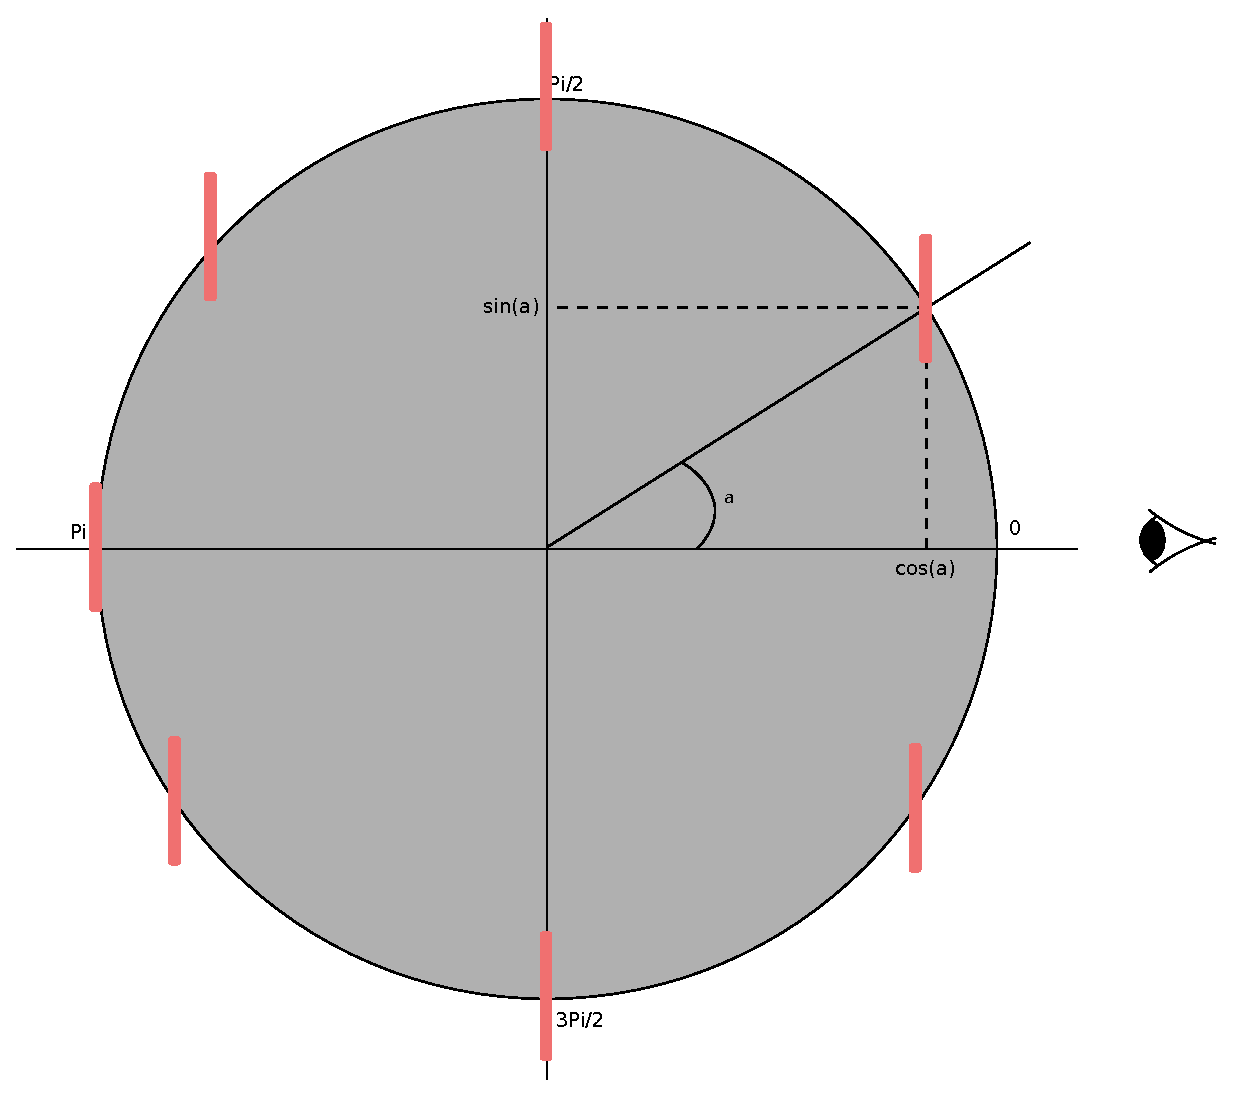
\includegraphics[width=8cm]{trigo.eps}
\end{frame}


\begin{frame}[fragile]{Rappel trigo}
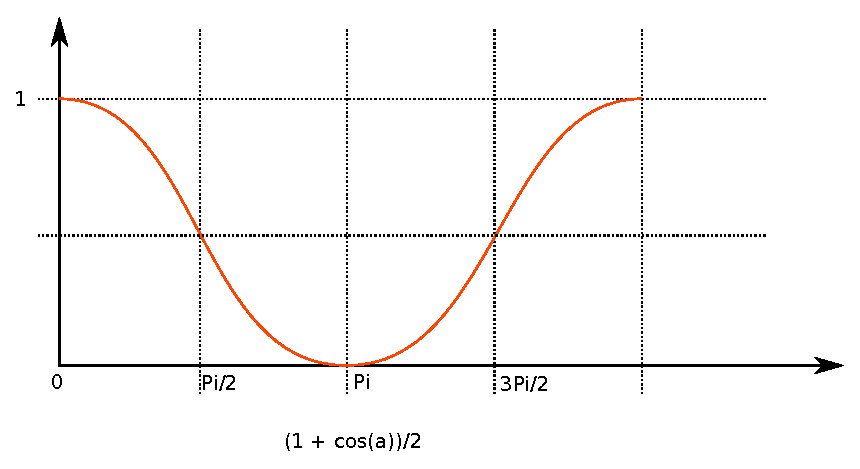
\includegraphics[width=8cm]{cosa.eps}
\end{frame}

\begin{frame}[fragile]{Rappel trigo}
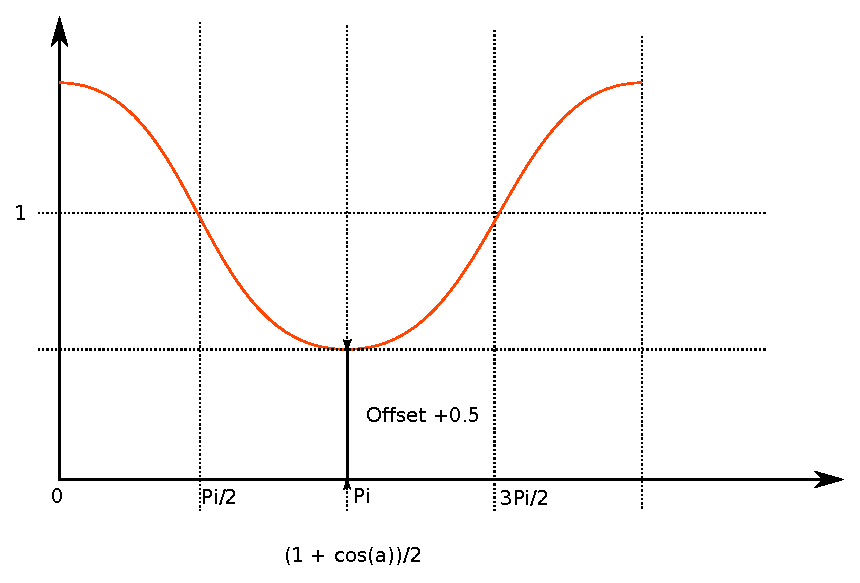
\includegraphics[width=8cm]{cosb.eps}
\end{frame}

\begin{frame}[fragile]{Facteur d'echelle des pochettes}
Les pochettes sont soumis a un facteur multiplicateur. La taille des pochettes varie entre 
0.5 x taille et 1.5 x taille.\\
\begin{lstlisting}
scale = 0.5 + (1.0 + cos(item->angle + t)) / 2.0;
...
w = ICON_SIZE_W * scale;
h = ICON_SIZE_H * scale;
\end{lstlisting}
\end{frame}

\begin{frame}[fragile]{Position en X}
La position des pochettes sur l'axe X est la projection des pochettes sur un plan. La position du centre des pochettes est donc fonction du sinus de l'angle.
\begin{lstlisting}
x = WIDTH / 2.0 + (sin(item->angle + t) * (WIDTH / 2.0)) - ICON_SIZE_W  / 2.0;
\end{lstlisting}
\end{frame}

\begin{frame}[fragile]{Position en Y}
La position en y pourrait être calcullée en fonction du cosinus de l'angle. On choisis ici un calcul plus simple en réutilisant la valeur de scale calculée précédement.
\begin{lstlisting}
y =  128 * scale;
\end{lstlisting}
\end{frame}

\begin{frame}[fragile]{Probléme de positionnement en z}
Les pochettes sont maintenant bien positionnées, mais ne sont pas ordonnées correctement, visuellement certaines devraient se retrouver derriére certaines autres.\\
Pour positionner correctement les pochettes nous allons utiliser le scale de chaque pochette.\\
Plus le scale est faible, plus la pochette et loin.\\
Nous trions donc la liste des objets en fonction du scale a l'aide de la fonction eina\_list\_sorted\_insert.\\
Puis on parcours la liste est on ordonne en utilisant evas\_object\_raise.
\end{frame}

\begin{frame}[fragile]{Fonction de tri}
\begin{lstlisting}
static int _compare_z(const void *data1, const void *data2)
{
    int d1 = evas_object_data_get(data1, "scale");
    int d2 = evas_object_data_get(data2, "scale");

    if (d1 > d2)
        return 1;
    else if (d1 < d2)
        return -1;
    else
        return 0;
}
...
z = eina_list_sorted_insert(z, _compare_z, item->obj);
...
EINA_LIST_FREE(z, obj)
    evas_object_raise(obj);
\end{lstlisting}
\end{frame}

\begin{frame}[fragile]{Animons le tout}
Crééons un ecore animator, qui va executer une callback au framerate défini dans ecore, par défaut à 30FPS.
\begin{lstlisting}
ecore_animator_add(_anim_cb, NULL);
\end{lstlisting}
la fonction \_anim prends maintenant un paramétre de type double : t. Ce parramétre est le temps courrant, ce qui permet d'animer notre carrousel en ajoutant cette valeur a l'angle des objets dans les calculs de cosinus et sinus.
\begin{lstlisting}
static Eina_Bool
_anim_cb(void *data)
{
    _anim(ecore_loop_time_get());
    return EINA_TRUE;
}
\end{lstlisting}
\end{frame}


\end{document}
